\documentclass[11pt]{article}
\usepackage{fullpage}
\usepackage{amsmath,amsthm,amssymb,amsfonts,multirow}
\usepackage{mathtools}
\usepackage{graphicx}
\usepackage{xcolor}
\usepackage{float}
%\usepackage{enumerate}
\usepackage[shortlabels, inline]{enumitem}
\usepackage{textcomp}
\usepackage{hyperref}
\usepackage{comment}

\usepackage{listings}
\lstset{language=Python, numbers=left, basicstyle=\ttfamily, keywordstyle=\color{blue}, showstringspaces=false}

\usepackage[style=alphabetic-verb]{biblatex}
% \bibliography{Problems/ref.bib}

\newcommand{\N}{\mathbb{N}}
\newcommand{\Z}{\mathbb{Z}}
\newcommand{\Q}{\mathbb{Q}}
\newcommand{\R}{\mathbb{R}}
\newcommand{\C}{\mathcal{C}}
\newcommand{\K}{\mathbb{K}}
\renewcommand{\div}{\mid}
\newcommand{\ndiv}{\nmid}
\newcommand{\E}{\mathbb{E}}
\newcommand{\I}{\mathbb{I}}
\newcommand{\F}{\mathcal{F}}

\DeclareMathOperator{\id}{Id}
\DeclareMathOperator{\tr}{Tr}
\DeclareMathOperator*{\argmax}{arg\,max}
\DeclareMathOperator*{\argmin}{arg\,min}
\DeclareMathOperator{\lcm}{lcm}
\DeclareMathOperator{\spn}{span}
\DeclareMathOperator{\acosh}{acosh}

\DeclarePairedDelimiter{\floor}{\lfloor}{\rfloor}
\DeclarePairedDelimiter{\ceil}{\lceil}{\rceil}
\DeclarePairedDelimiter{\abs}{\lvert}{\rvert}

\newcommand{\subtag}[1]{\tag{\theparentequation#1}}

\renewcommand{\vec}[1]{\mathbf{#1}}

\usepackage{subfiles}
\usepackage{subcaption}
\makeatletter
\newcommand\nocaption{
    \renewcommand\p@subfigure{}
    \renewcommand{\thesubfigure}{\arabic{figure}\alph{subfigure}}
}
\makeatother


\newenvironment{problem}[2][Question]{\begin{trivlist}
\item[\hskip \labelsep {\bfseries #1}\hskip \labelsep {\bfseries #2.}]}{\end{trivlist}}

\newenvironment{solution}{%
  \begin{proof}[\textbf{Solution}]$ $\par\nobreak\ignorespaces
}{%
  \end{proof}
}

\theoremstyle{definition}
\newtheorem{definition}{Definition}
\newtheorem{theorem}{Theorem}
\newtheorem{lemma}{Lemma}

\hypersetup{
    colorlinks=true,
    linkcolor=blue,
    filecolor=magenta,      
    urlcolor=cyan,
    pdftitle={Overleaf Example},
    pdfpagemode=FullScreen,
    }


\title{Intro to Computational Mathematics: Section 11}
\date{November 2025}

\begin{document}
\maketitle

\begin{problem}{6.1.1}
For each IVP, determine whether the problem satisfies the conditions of \href{https://fncbook.com/basics/#theorem-depic}{Theroem 6.1.2}. If so, determine the smallest possible value for $L$.
\begin{enumerate}[(a)]
\item $f(t, u) = 3u$, $0 \leq t \leq 1$
\item $f(t, u) = -t\sin(u)$, $0 \leq t \leq 5$
\item $f(t, u) = -(1 + t^2)u^2$, $1 \leq t \leq 3$
\item $f(t, u) = \sqrt{u}$, $0 \leq t \leq 1$
\end{enumerate}
\end{problem}
\begin{solution}
Theorem 6.1.2 tells us that a unique solution exists if $\frac{\partial f}{\partial u}$ exists and is bounded by a constant $L$ for all $t, u$ in the relevant domains. The question then is to determine if the relevant partial derivatives exist and remain bounded.
\begin{enumerate}[(a)]
    \item $\frac{\partial f}{\partial u} = 3$, which is bounded by $L = 3$.
    \item $\frac{\partial f}{\partial u} = -t\cos(u)$ which is bounded by $L = 5$.
    \item $\frac{\partial f}{\partial u} = -2(1 + t^2)u$ which is not bounded by a constant since $u$ can be arbitrarily large.
    \item $\frac{\partial f}{\partial u} = \frac{1}{2\sqrt{u}}$ which is not defined at $u = 0$ nor bounded in the domain $u \in (0, \infty)$.
\end{enumerate}
\end{solution}



\begin{problem}{6.1.2}
For each ODE in the preceding problem, assume that $u$ is initially equal to $1$ on the given interval. Solve the resulting IVP as in \href{https://fncbook.com/basics/#demo-basics-first}{Example 6.1.2}, and make a plot of the solution.
\end{problem}
\begin{solution}
The following code produces the desired results.
\begin{lstlisting}
import numpy as np
from scipy.integrate import solve_ivp
import matplotlib.pyplot as plt

f_a = lambda t, u: 3*u
f_b = lambda t, u: -t * np.sin(u)
f_c = lambda t, u: -(1 + t**2) * u**2
f_d = lambda t, u: np.sqrt(u)

u0 = np.array([1.0])
sol_a = solve_ivp(f_a, [0, 1], u0, t_eval=np.linspace(0, 1, 200))
sol_b = solve_ivp(f_b, [0, 5], u0, t_eval=np.linspace(0, 5, 200))
sol_c = solve_ivp(f_c, [1, 3], u0, t_eval=np.linspace(1, 3, 200))
sol_d = solve_ivp(f_d, [0, 1], u0, t_eval=np.linspace(0, 1, 200))

plt.plot(sol_a.t, sol_a.y[0, :], label='a')
plt.plot(sol_b.t, sol_b.y[0, :], label='b')
plt.plot(sol_c.t, sol_c.y[0, :], label='c')
plt.plot(sol_d.t, sol_d.y[0, :], label='d')
plt.legend()
plt.xlabel("t")
plt.ylabel("u(t)")
plt.show()
\end{lstlisting}
Output:
\begin{center}
    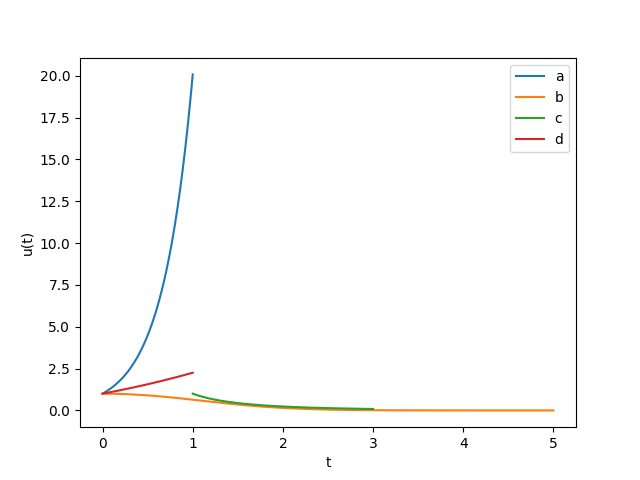
\includegraphics[width=0.8\textwidth]{6.1.2_fig.png}
\end{center}
\end{solution}



\begin{problem}{6.1.7}
Experimental evidence (see \href{https://doi.org/10.1007/BF00609587}{Newton et al. (1981)}) shows that a 300-mg oral dose of caffeine, such as might be found in a large mug of drip-brewed coffee, creates a concentration of about 8 $\mu g/mL$ in blood plasma. This boost is followed by first-order kinetics with a half-life of about 6 hours (although this rate can vary a great deal from person to person). We can model the caffeine concentration due to one drink taken over half an hour via
$$x'(t) = -kx + C(t), \qquad x(0) = 0,$$
where $k = \log(2)/6$ and
$$C(t) = \begin{cases}16, \quad 0 \leq t \leq 0.5, \\ 0, \quad t > 0.5.\end{cases}$$
Solve the IVP and make a plot of the caffeine concentration for 12 hours. Then change $k = \log(2)/8$ (half-life of 8 hours) and plot the solution again.
\end{problem}
\begin{solution}
The following code produces the desired output:
\begin{lstlisting}
import numpy as np
from scipy.integrate import solve_ivp
import matplotlib.pyplot as plt


k = np.log(2)/6
C = lambda t: 16 if t <= 0.5 else 0
f = lambda t, x: -k*x + C(t)

k_2 = np.log(2)/8
f_2 = lambda t, x: -k_2*x + C(t)

x0 = np.array([0.0])
sol_a = solve_ivp(f, [0, 12], x0, t_eval=np.linspace(0, 12, 200))
sol_b = solve_ivp(f_2, [0, 12], x0, t_eval=np.linspace(0, 12, 200))

plt.plot(sol_a.t, sol_a.y[0, :], label='a')
plt.plot(sol_b.t, sol_b.y[0, :], label='b')
plt.legend()
plt.xlabel("t")
plt.ylabel("x(t)")
plt.title("Caffeine Concentration over Time")
plt.show()
\end{lstlisting}
Output:
\begin{center}
    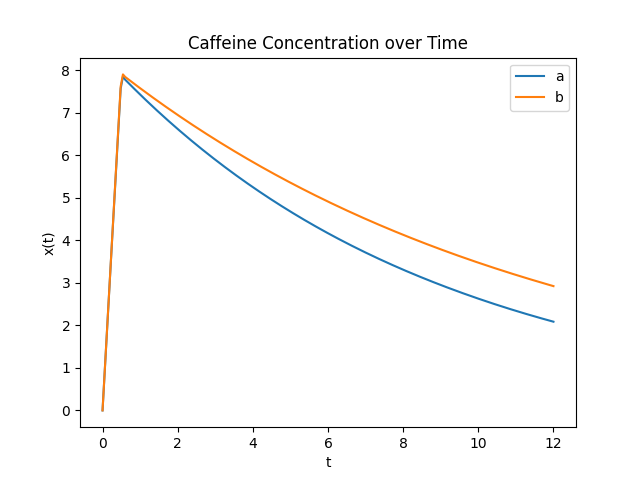
\includegraphics[width=0.8\textwidth]{6.1.7_fig.png}
\end{center}
\end{solution}



\begin{problem}{Q2}
Consider numerically integrating a function $f\colon \mathbb{R}\rightarrow \mathbb{R}$ from $0$ to $1$, given the following:
\begin{align*}
    f(0) &= 1,\\
    f(1/2) &= -1,\\
    f(1) &= 5.    
\end{align*}
\begin{enumerate}[(a)]
\item Given this, compute the best linear function $x\mapsto ax+b$ approximating $f$ via least squares.\\
Estimate the value of the integral by integrating this approximation.
\item Compute the trapezoid integration approximation for this with $n=2$ and with $n=4$ given the additional function evaluations $f(1/4) = -1$ and $f(3/4) = 1$.
\item From these, compute the Simpson's Extrapolation approximation for this integral.
\item If in addition to $0,1/4,1/2,3/4,1$, you could evaluate $f$ at two more points in $[0,1]$ to give a more accurate estimate, where would you select? Why?
\end{enumerate}
\end{problem}
\begin{solution}
\begin{enumerate}[(a)]
\item Assuming a linear approximation, we can represent $f$ by the equation $f \approx ax + b$. Since we want to simultaneously satisfy this at:
\begin{align*}
    1 &= a(0) + b \\
    -1 &= a(1/2) + b \\
    5 &= a(1) + b
\end{align*}
This is an overdetermined system, which we can find a best fit for by trying to minimize the equation:
$$\left\|\begin{bmatrix*}0 & 1 \\ 1/2 & 1 \\ 1 & 1\end{bmatrix*}\begin{bmatrix*}a \\ b\end{bmatrix*} - \begin{bmatrix*}1 \\ - 1 \\ 5\end{bmatrix*}\right\|.$$
This overdetermined system is solved using the normal equations: $A^T A x = A^T b$. That is, we wish to solve:
\begin{align*}
    \begin{bmatrix*}0 & 1 \\ 1/2 & 1 \\ 1 & 1\end{bmatrix*}^T\begin{bmatrix*}0 & 1 \\ 1/2 & 1 \\ 1 & 1\end{bmatrix*}\begin{bmatrix*}a \\ b\end{bmatrix*} &= \begin{bmatrix*}0 & 1 \\ 1/2 & 1 \\ 1 & 1\end{bmatrix*}^T \begin{bmatrix*}1 \\ - 1 \\ 5\end{bmatrix*} \\
    \begin{bmatrix*}0 & 1/2 & 1 \\ 1 & 1 & 1\end{bmatrix*}\begin{bmatrix*}0 & 1 \\ 1/2 & 1 \\ 1 & 1\end{bmatrix*}\begin{bmatrix*}a \\ b\end{bmatrix*} &= \begin{bmatrix*}0 & 1/2 & 1 \\ 1 & 1 & 1\end{bmatrix*} \begin{bmatrix*}1 \\ - 1 \\ 5\end{bmatrix*} \\
    \begin{bmatrix*}5/4 & 3/2 \\ 3/2 & 3\end{bmatrix*} \begin{bmatrix*}a \\ b\end{bmatrix*} &= \begin{bmatrix*} 9/2 \\ 5 \end{bmatrix*} \\
\end{align*}
We can solve this linear system using the LU decomposition:
\begin{align*}
    \begin{bmatrix*}5/4 & 0 \\ 3/2 &  6/5\end{bmatrix*}\begin{bmatrix*}1 & 6/5 \\ 0 & 1\end{bmatrix*}\begin{bmatrix*}a \\ b\end{bmatrix*} &= \begin{bmatrix*} 9/2 \\ 5 \end{bmatrix*}
\end{align*}
Substituting $Ux = y$, we solve $Ly = b$:
\begin{align*}
    \begin{bmatrix*}5/4 & 0 \\ 3/2 &  6/5\end{bmatrix*}y &= \begin{bmatrix*} 9/2 \\ 5 \end{bmatrix*} \\
    y &= \begin{bmatrix*}18/5 \\ -1/3\end{bmatrix*} \\
    \begin{bmatrix*}1 & 6/5 \\ 0 & 1\end{bmatrix*}\begin{bmatrix*}a \\ b\end{bmatrix*} &= \begin{bmatrix*}18/5 \\ -1/3\end{bmatrix*} \\
    \begin{bmatrix*}a \\ b\end{bmatrix*} &= \begin{bmatrix*}4 \\ -1/3\end{bmatrix*}
\end{align*}
Thus the best linear approximation is given by $f(x) = 4x - 1/3$. Integrating $\int_0^1 4x - 1/3 \, dx = 2x^2 - (1/3)x \bigg\vert_0^1 = 5/3$.
\item The trapezoid approximation rule is given by: $$\int_a^b f(x) \, dx \approx \frac{b - a}{n}[\frac{1}{2}f(x_0) + f(x_1) + \ldots + f(x_{n-1}) + \frac{1}{2}f(x_n)].$$
Plugging in $n = 2$, we get:
\begin{align*}
    \int_0^1 f(x) \, dx &\approx T_f(2) \\
    &= \frac{1 - 0}{2}[\frac{1}{2}f(0) + f(\frac{1}{2}) + \frac{1}{2}f(1)] \\
    &= \frac{1}{2}[\frac{1}{2}(1) + (-1) + \frac{1}{2}(5)] \\
    &= 1
\end{align*}
Plugging in $n = 4$, we get:
\begin{align*}
    \int_0^1 f(x) \, dx &\approx T_f(4) \\
    &=\frac{1 - 0}{4}[\frac{1}{2}f(0) + f(\frac{1}{4}) + f(\frac{1}{2}) + f(\frac{3}{4}) +  \frac{1}{2}f(1)] \\
    &= \frac{1}{4}[\frac{1}{2}(1) + (-1) + (-1) + (1) + \frac{1}{2}(5)] \\
    &= 1
\end{align*}
\item Simpsons Rule combines $T_f(2)$ and $T_f(4)$ using linear algebra to remove the coefficients corresponding to the second-order error given by Taylor's Theorem. Thus $S_f(4) = \frac{1}{3}[4T_f(4) - T_f(2)]$ gives the better approximation:
\begin{align*}
    S_f(4) &= \frac{1}{3}[4T_f(4) - T_f(2)] \\
    &= \frac{1}{3}[4(1) - 1] \\
    &= 1
\end{align*}
\item The remaining error after computing $S_f(4)$ is proportional to the fourth derivative term, so it makes the most sense to better approximate the function in regions where the fourth derivative is large: i.e. we should consider $x = 5/8, 7/8$ as the most reasonable points for improving the accuracy of the numerical integration.
\end{enumerate}
\end{solution}

\end{document}
